\chapter{Monai Valley experiment (monai\_valley)}

\section{Purpose}

This test case redoes the monai valley experiment from Costas E Synolakis
(p.45, 3.4) \cite{Costas2007}.

\section{Description}

The configuration is a 5.5~m long and 3.4~m wide rectangle.

\subsection{Mesh and geometry}

The mesh is made of 25,553 elements and 12,989 nodes
(see Figure~\ref{fig:monai:mesh}).

\begin{figure}[H]
\centering
\includegraphicsmaybe{[width=.9\textwidth]}{../img/Mesh.png}
\caption{Mesh of the study.}
\label{fig:monai:mesh}
\end{figure}

Figure~\ref{fig:monai:bathy} shows the bathymetry of the study.

\begin{figure}[H]
\centering
\includegraphicsmaybe{[width=.9\textwidth]}{../img/Bathy.png}
\caption{Bathymetry of the study.}
\label{fig:monai:bathy}
\end{figure}

\subsection{Boundary}

Figure~\ref{fig:monai:boundaries} shows the boundaries of the study and the
incident wave.

\begin{figure}[H]
\centering
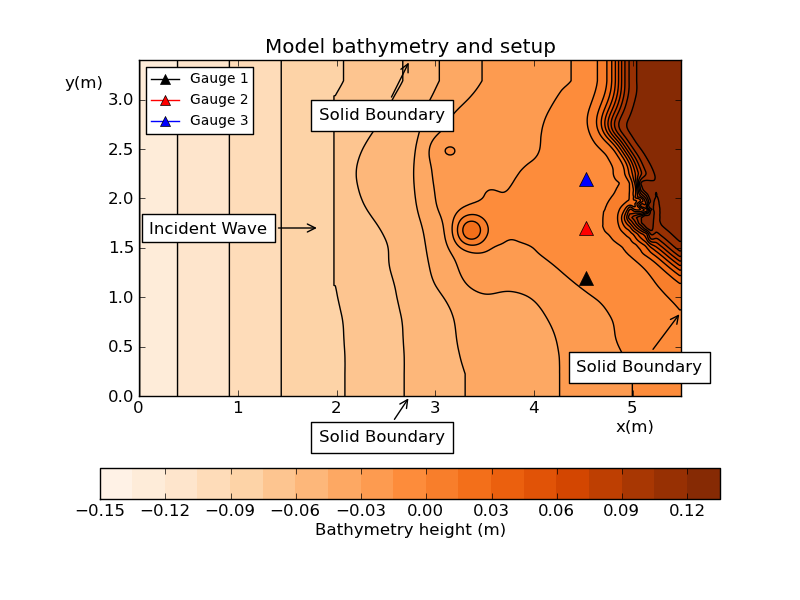
\includegraphics[width=.6\textwidth]{img/boundaries.png}
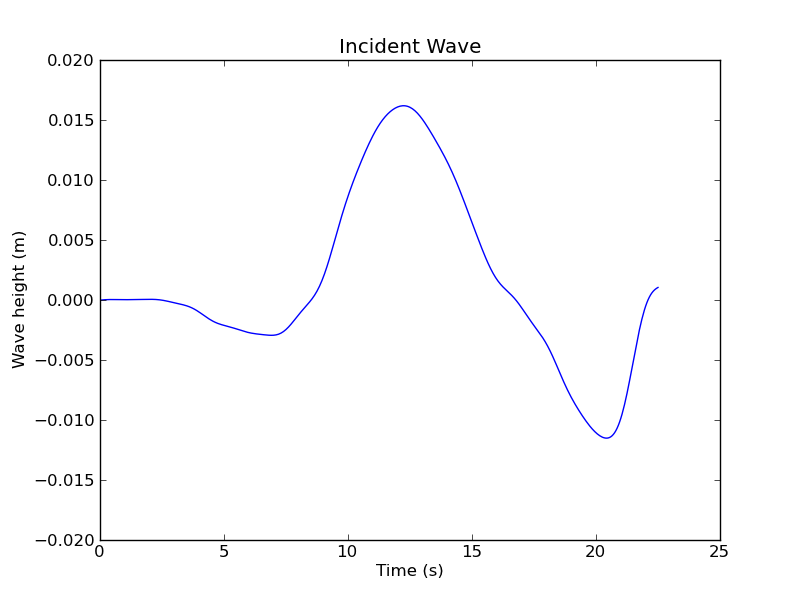
\includegraphics[width=.6\textwidth]{img/wave.png}
\caption{Boundaries of the study.}
\label{fig:monai:boundaries}
\end{figure}

Chézy's friction law is used for the bottom with a friction coefficient equal
to 180~m$^{1/2}$/s.

\subsection{Physical parameters}

Constant viscosity equal to 0~m$^2$/s is used as turbulence model.

\subsection{Numerical parameters}
\begin{itemize}
\item Type of element: P1 triangle for $h$ and for velocity,
\item Solver: GMRES,
\item Accuracy: $10^{-6}$,
\item Finite volume scheme: Kinetic order 2.
\end{itemize}

Time data:
\begin{itemize}
%\item Time step: 0.000~5~s,
\item Desired Courant number = 0.9,
\item Simulation duration: 22.5~s.
\end{itemize}

\section{Results}

Figure~\ref{fig:monai:vel} shows the velocity vectors.

\begin{figure}[H]
\centering
\includegraphicsmaybe{[width=.9\textwidth]}{../img/Velocity.png}
\caption{Velocity.}
\label{fig:monai:vel}
\end{figure}

Figure~\ref{fig:monai:FreeSurf} shows the free surface elevation.

\begin{figure}[H]
\centering
\includegraphicsmaybe{[width=.9\textwidth]}{../img/FreeSurface.png}
\caption{Free surface elevation.}
\label{fig:monai:FreeSurf}
\end{figure}

We compare the model and experiment free surface at gauges 1,2 and 3.

Figure~\ref{fig:monai:res} shows the comparison with the benchmark data.

\begin{figure}[H]
\centering
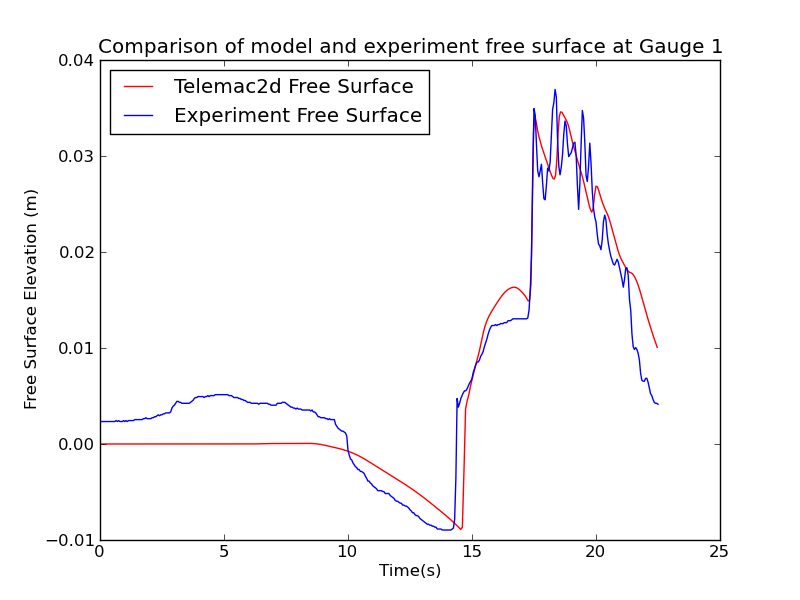
\includegraphics[width=.8\textwidth]{img/res_g1.png}
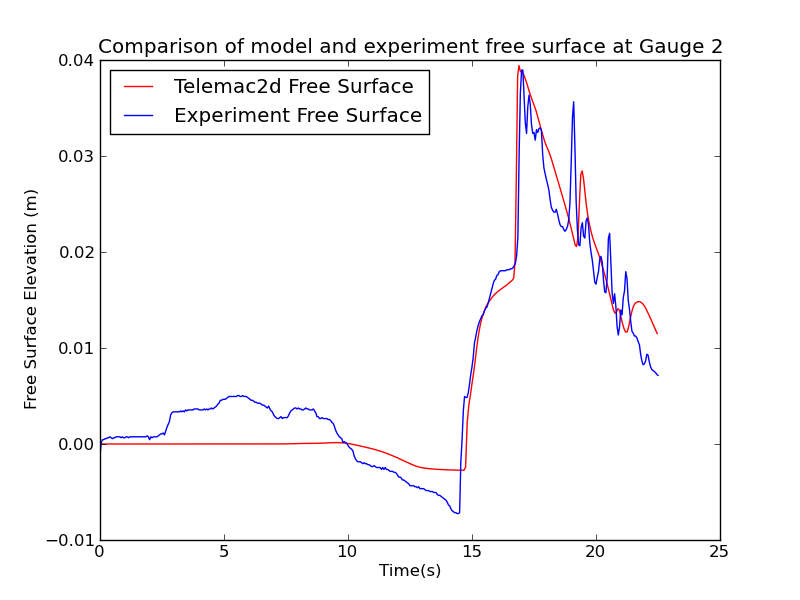
\includegraphics[width=.8\textwidth]{img/res_g2.png}
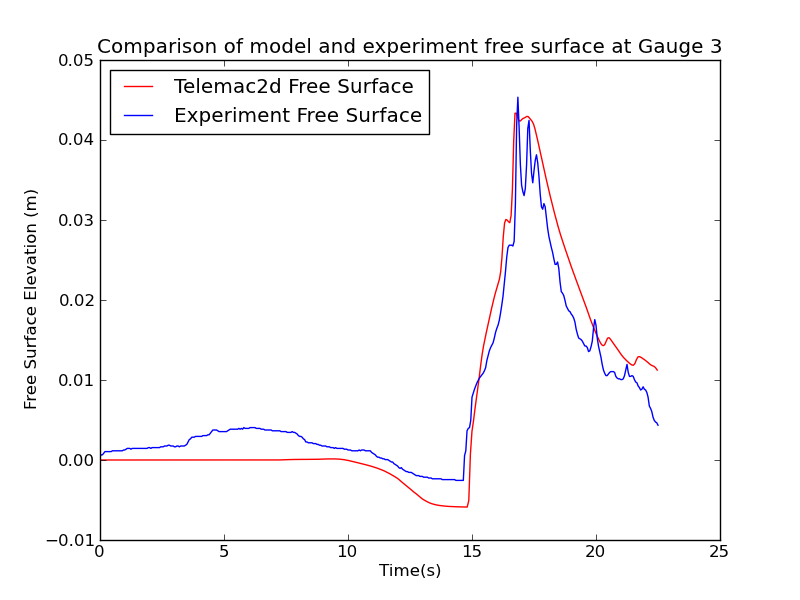
\includegraphics[width=.8\textwidth]{img/res_g3.png}
\caption{Comparaison of the results.}
\label{fig:monai:res}
\end{figure}
